\PassOptionsToPackage{unicode=true}{hyperref} % options for packages loaded elsewhere
\PassOptionsToPackage{hyphens}{url}
%
\documentclass[english,man,floatsintext]{apa6}
\usepackage{lmodern}
\usepackage{amssymb,amsmath}
\usepackage{ifxetex,ifluatex}
\usepackage{fixltx2e} % provides \textsubscript
\ifnum 0\ifxetex 1\fi\ifluatex 1\fi=0 % if pdftex
  \usepackage[T1]{fontenc}
  \usepackage[utf8]{inputenc}
  \usepackage{textcomp} % provides euro and other symbols
\else % if luatex or xelatex
  \usepackage{unicode-math}
  \defaultfontfeatures{Ligatures=TeX,Scale=MatchLowercase}
\fi
% use upquote if available, for straight quotes in verbatim environments
\IfFileExists{upquote.sty}{\usepackage{upquote}}{}
% use microtype if available
\IfFileExists{microtype.sty}{%
\usepackage[]{microtype}
\UseMicrotypeSet[protrusion]{basicmath} % disable protrusion for tt fonts
}{}
\IfFileExists{parskip.sty}{%
\usepackage{parskip}
}{% else
\setlength{\parindent}{0pt}
\setlength{\parskip}{6pt plus 2pt minus 1pt}
}
\usepackage{hyperref}
\hypersetup{
            pdftitle={Supplemental information for Parent material and climate interact to control soil C dynamics through the development of poorly crystalline minerals},
            pdfauthor={Jeffrey Beem-Miller1, Craig Rasmussen2, Alison M. Hoyt1,3, Marion Schrumpf1, Georg Guggenberger4, \& Susan Trumbore1},
            pdfborder={0 0 0},
            breaklinks=true}
\urlstyle{same}  % don't use monospace font for urls
\usepackage{graphicx,grffile}
\makeatletter
\def\maxwidth{\ifdim\Gin@nat@width>\linewidth\linewidth\else\Gin@nat@width\fi}
\def\maxheight{\ifdim\Gin@nat@height>\textheight\textheight\else\Gin@nat@height\fi}
\makeatother
% Scale images if necessary, so that they will not overflow the page
% margins by default, and it is still possible to overwrite the defaults
% using explicit options in \includegraphics[width, height, ...]{}
\setkeys{Gin}{width=\maxwidth,height=\maxheight,keepaspectratio}
\setlength{\emergencystretch}{3em}  % prevent overfull lines
\providecommand{\tightlist}{%
  \setlength{\itemsep}{0pt}\setlength{\parskip}{0pt}}
\setcounter{secnumdepth}{0}

% set default figure placement to htbp
\makeatletter
\def\fps@figure{htbp}
\makeatother

% Manuscript styling
\usepackage{upgreek}
\captionsetup{font=singlespacing,justification=justified}

% Table formatting
\usepackage{longtable}
\usepackage{lscape}
% \usepackage[counterclockwise]{rotating}   % Landscape page setup for large tables
\usepackage{multirow}		% Table styling
\usepackage{tabularx}		% Control Column width
\usepackage[flushleft]{threeparttable}	% Allows for three part tables with a specified notes section
\usepackage{threeparttablex}            % Lets threeparttable work with longtable

% Create new environments so endfloat can handle them
% \newenvironment{ltable}
%   {\begin{landscape}\centering\begin{threeparttable}}
%   {\end{threeparttable}\end{landscape}}
\newenvironment{lltable}{\begin{landscape}\centering\begin{ThreePartTable}}{\end{ThreePartTable}\end{landscape}}

% Enables adjusting longtable caption width to table width
% Solution found at http://golatex.de/longtable-mit-caption-so-breit-wie-die-tabelle-t15767.html
\makeatletter
\newcommand\LastLTentrywidth{1em}
\newlength\longtablewidth
\setlength{\longtablewidth}{1in}
\newcommand{\getlongtablewidth}{\begingroup \ifcsname LT@\roman{LT@tables}\endcsname \global\longtablewidth=0pt \renewcommand{\LT@entry}[2]{\global\advance\longtablewidth by ##2\relax\gdef\LastLTentrywidth{##2}}\@nameuse{LT@\roman{LT@tables}} \fi \endgroup}

% \setlength{\parindent}{0.5in}
% \setlength{\parskip}{0pt plus 0pt minus 0pt}

% \usepackage{etoolbox}
\makeatletter
\patchcmd{\HyOrg@maketitle}
  {\section{\normalfont\normalsize\abstractname}}
  {\section*{\normalfont\normalsize\abstractname}}
  {}{\typeout{Failed to patch abstract.}}
\patchcmd{\HyOrg@maketitle}
  {\section{\protect\normalfont{\@title}}}
  {\section*{\protect\normalfont{\@title}}}
  {}{\typeout{Failed to patch title.}}
\makeatother
\shorttitle{Supplemental information}
\DeclareDelayedFloatFlavor{ThreePartTable}{table}
\DeclareDelayedFloatFlavor{lltable}{table}
\DeclareDelayedFloatFlavor*{longtable}{table}
\makeatletter
\renewcommand{\efloat@iwrite}[1]{\immediate\expandafter\protected@write\csname efloat@post#1\endcsname{}}
\makeatother
\usepackage{lineno}

\linenumbers
\usepackage{csquotes}
\usepackage[titles]{tocloft}
\cftpagenumbersoff{figure}
\renewcommand{\cftfigpresnum}{\itshape\figurename\enspace}
\renewcommand{\cftfigaftersnum}{.\space}
\setlength{\cftfigindent}{0pt}
\setlength{\cftafterloftitleskip}{0pt}
\settowidth{\cftfignumwidth}{Figure 10.\qquad}
\cftpagenumbersoff{table}
\renewcommand{\cfttabpresnum}{\itshape\tablename\enspace}
\renewcommand{\cfttabaftersnum}{.\space}
\setlength{\cfttabindent}{0pt}
\setlength{\cftafterloftitleskip}{0pt}
\settowidth{\cfttabnumwidth}{Table 10.\qquad}
\ifnum 0\ifxetex 1\fi\ifluatex 1\fi=0 % if pdftex
  \usepackage[shorthands=off,main=english]{babel}
\else
  % load polyglossia as late as possible as it *could* call bidi if RTL lang (e.g. Hebrew or Arabic)
  \usepackage{polyglossia}
  \setmainlanguage[]{english}
\fi

\title{Supplemental information for Parent material and climate interact to control soil C dynamics through the development of poorly crystalline minerals}
\author{Jeffrey Beem-Miller\textsuperscript{1}, Craig Rasmussen\textsuperscript{2}, Alison M. Hoyt\textsuperscript{1,3}, Marion Schrumpf\textsuperscript{1}, Georg Guggenberger\textsuperscript{4}, \& Susan Trumbore\textsuperscript{1}}
\date{}


\affiliation{\vspace{0.5cm}\textsuperscript{1} Department of Biogeochemical Processes, Max Planck Institute for Biogeochemistry, Jena, Germany\\\textsuperscript{2} Department of Environmental Science, The University of Arizona, Tucson, AZ, USA\\\textsuperscript{3} Department of Earth System Science Science, Stanford University, Stanford, CA, USA\\\textsuperscript{4} Institute of Soil Science, Leibniz University Hannover, Hannover, Germany}

\begin{document}
\maketitle

\hypertarget{soil-carbon}{%
\section{Soil carbon}\label{soil-carbon}}

We did not observe clear trends in soil carbon concentration over time for the majority of sites, making us confident that most sites are at steady-state with regards to carbon stock changes (\textbf{Fig. \ref{fig:plot-C-timeseries}}). Although we did observe substantial variation in some sites, this is likely due to spatial heterogeneity in soil C concentration that cannot be avoided when destructively resampling the same sites over time (\textbf{Fig. \ref{fig:plot-C-timeseries}}). However, we did observe significant trends in soil C concentration with time for a a few of the sites when considered by specific depth increments. However, a caveat here is that we did not account for potential differences in the mass of soil sampled over time, as we only considered depth-based increments. We observed the most significant changes at the soil surface, at three of the 9 sites, but only two sites showed significant changes at the 10-20cm depth, and only one of the soils showed changes at the deepest depth (\textbf{Table \ref{tab:pct-C-change-tbl}}). The soil at the cold climate andesite site was an outlier in that the soil C concentration showed a consistently significant increase for all depths over the study period (\textbf{Table \ref{tab:pct-C-change-tbl}}).



\begingroup\fontsize{10}{12}\selectfont

\begin{longtable}[t]{llrrrrr}
\caption{\label{tab:pct-C-change-tbl}Changes in soil C concentration (\%), 2001-2019. (Only signficant trends shown).}\\
\toprule
\multicolumn{5}{c}{ } & \multicolumn{2}{c}{95\% CI} \\
\cmidrule(l{3pt}r{3pt}){6-7}
Depth & Site & Trend & $SE$ & df & $lower$ & $upper$\\
\midrule
\endfirsthead
\caption[]{\label{tab:pct-C-change-tbl}Changes in soil C concentration (\%), 2001-2019. (Only signficant trends shown). \textit{(continued)}}\\
\toprule
\multicolumn{5}{c}{ } & \multicolumn{2}{c}{95\% CI} \\
\cmidrule(l{3pt}r{3pt}){6-7}
Depth & Site & Trend & $SE$ & df & $lower$ & $upper$\\
\midrule
\endhead

\endfoot
\bottomrule
\endlastfoot
 & andesite (warm) & -0.19 & 0.09 & 62 & -0.37 & -0.01\\
\nopagebreak
 & andesite (cold) & 0.20 & 0.10 & 62 & 0.01 & 0.40\\
\nopagebreak
\multirow[t]{-3}{*}{\raggedright\arraybackslash 0-10cm} & basalt (cold) & -0.43 & 0.09 & 62 & -0.61 & -0.25\\
\cmidrule{1-7}\pagebreak[0]
 & andesite (cold) & 0.23 & 0.06 & 62 & 0.12 & 0.35\\
\nopagebreak
\multirow[t]{-2}{*}{\raggedright\arraybackslash 10-20cm} & granite (warm) & 0.16 & 0.05 & 62 & 0.05 & 0.26\\
\cmidrule{1-7}\pagebreak[0]
20-30cm & andesite (cold) & 0.21 & 0.04 & 62 & 0.13 & 0.29\\*
\end{longtable}
\endgroup{}



\begin{figure}

{\centering 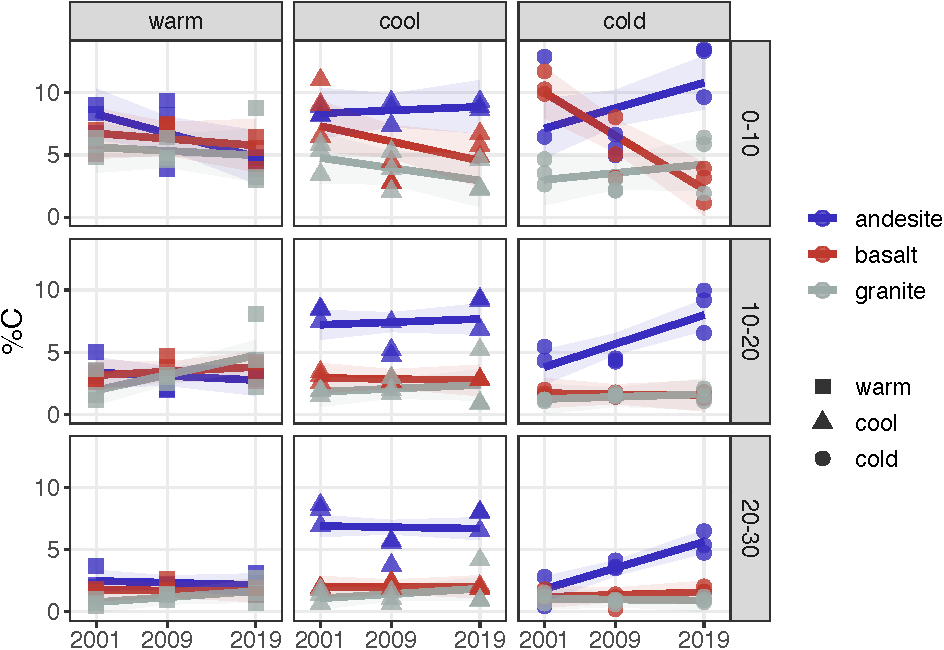
\includegraphics{sra-blk-inc-SI_files/figure-latex/plot-C-timeseries-1} 

}

\caption{Changes in soil C concentration, 2001-2019. Points show replicate profiles (n = 3); lines show marginal mean estimates of linear trends in soil C concentration with time; ribbons show 95\% CIs around trend estimates.}\label{fig:plot-C-timeseries}
\end{figure}

\hypertarget{respiration-fluxes}{%
\section{Respiration fluxes}\label{respiration-fluxes}}

\textbf{SI Figs. \ref{fig:plot-cmtv-flx-rates}} and \textbf{\ref{fig:plot-C-resp-rates-ts}}.

\begin{figure}

{\centering 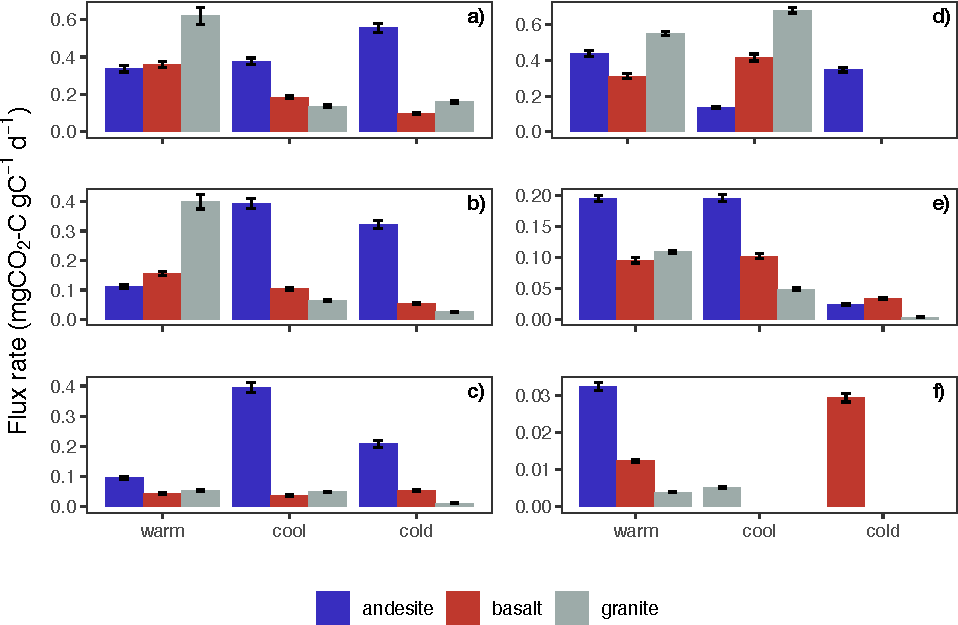
\includegraphics{sra-blk-inc-SI_files/figure-latex/plot-cmtv-flx-rates-1} 

}

\caption{Heterotrophic respiration rates from incubations of 2019 and 2001 samples. Panels a-c show 2019 data, and panels d-f show 2001 data. Panels in the top row (a, d) show the first depth increment for each year, middle row shows the second depth increment (b, e), and the bottom row shows the third depth increment (c, f). Columns show means for laboratory duplicates averaged over the whole incubation period; error bars ± 1 standard error of the mean. NB: Total CO\textsubscript{2} respired was controlled to be within 10,000 ppm (±1,000 ppm) for all samples; incubation duration varied between 4 and 40 days.}\label{fig:plot-cmtv-flx-rates}
\end{figure}



\begin{figure}

{\centering 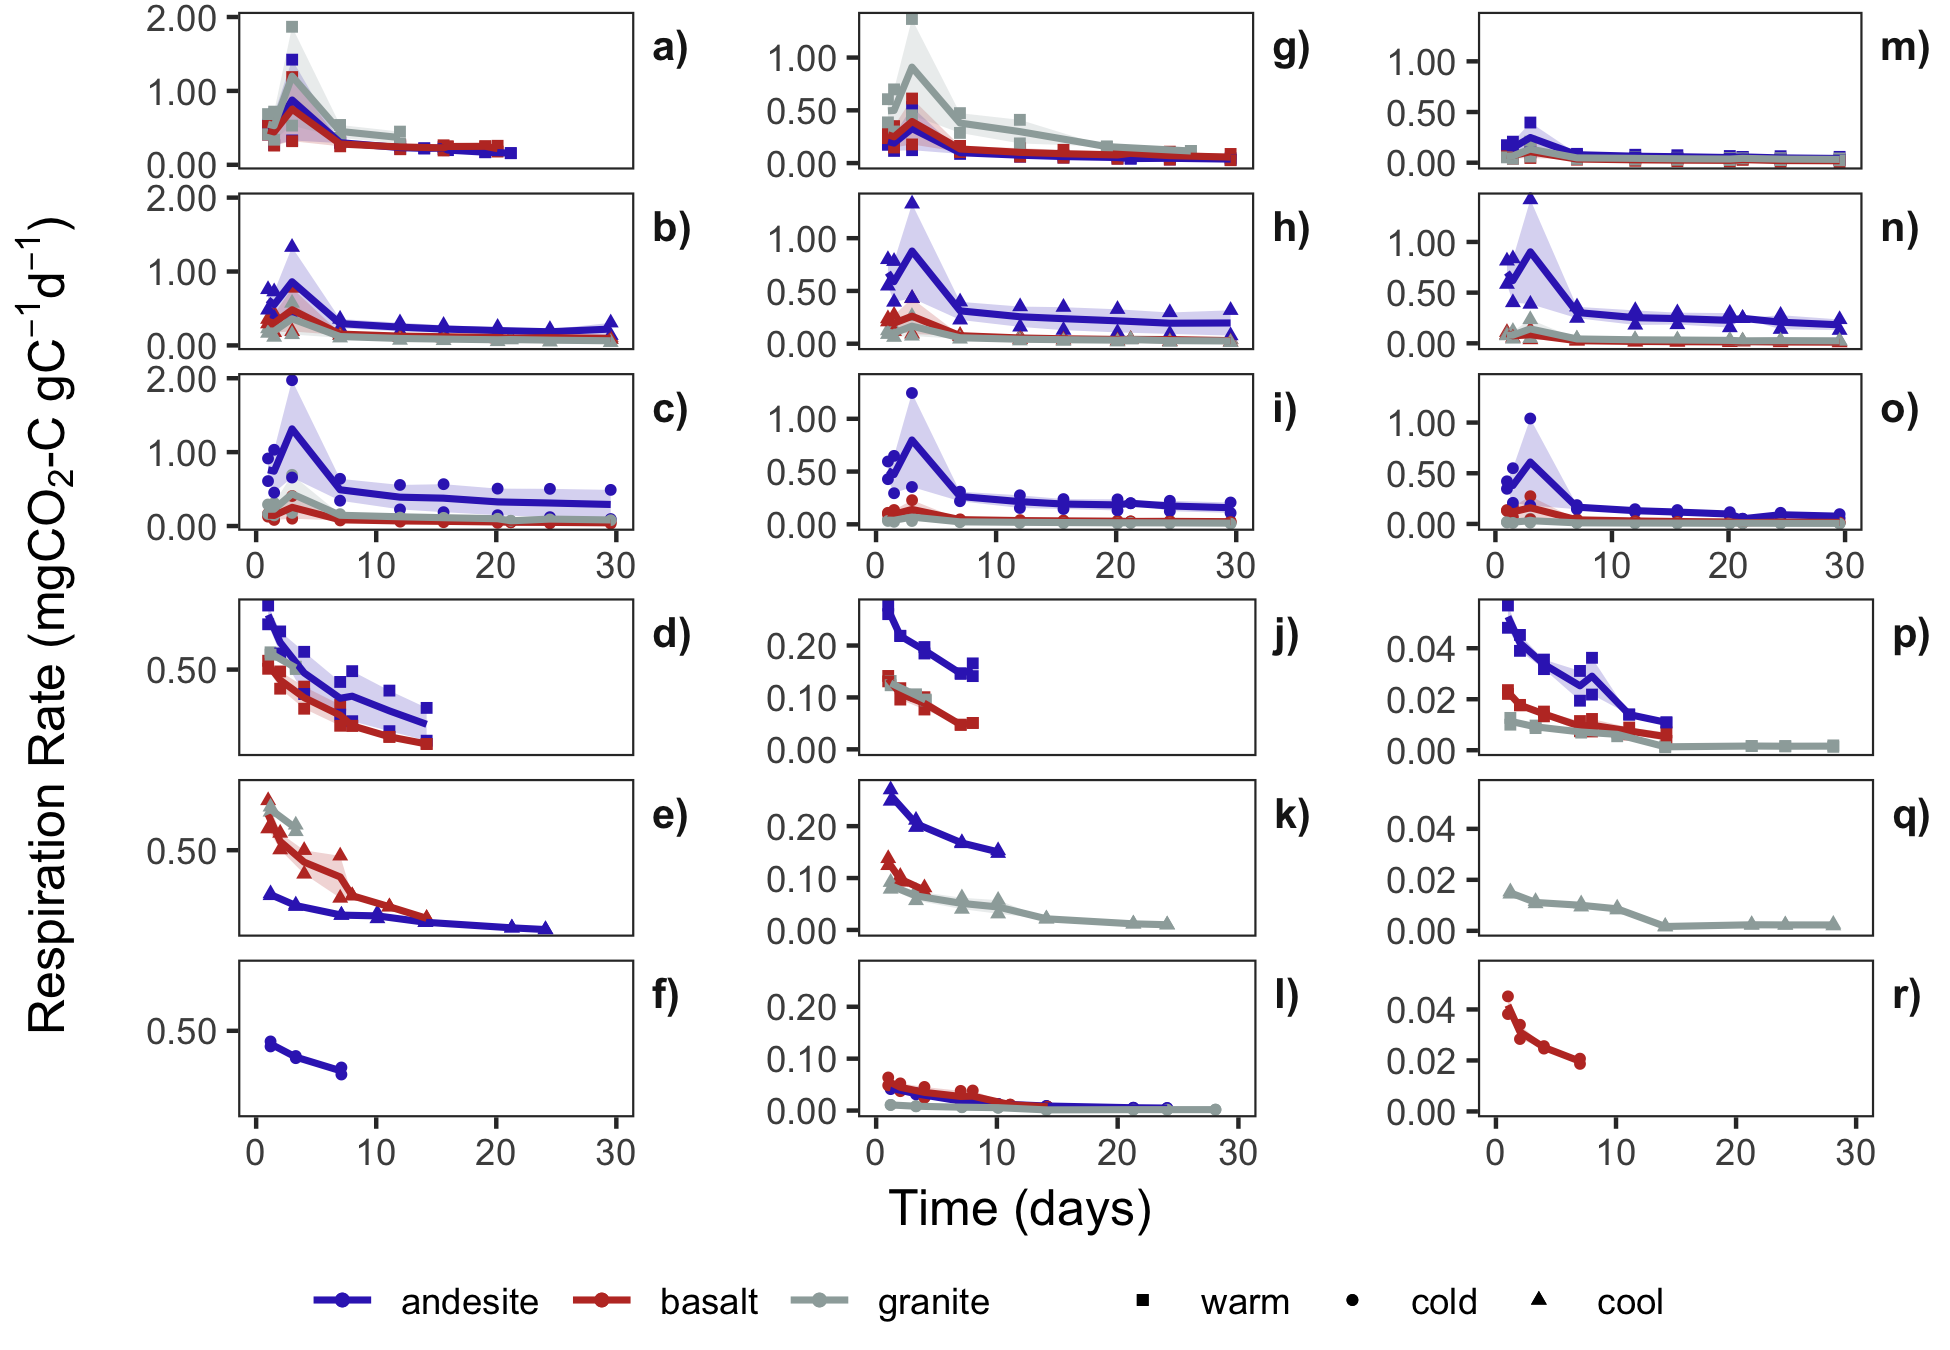
\includegraphics{sra-blk-inc-SI_files/figure-latex/plot-C-resp-rates-ts-1} 

}

\caption{Time series of heterotrophic respiration rates from incubations by depth and year (i.e.~samples from the same year and depth interval are plotted on the same scale). Rows correspond to climate zones, columns correspond to depths; leftmost column shows top depth, rightmost column shows deepest depth. Top set of panels (a-c, g-i, and m-o) show 2019 data, bottom set of panels (d-f, j-l, p-r) show 2001 data. Lines show means for laboratory duplicates; ribbon shows minimum and maximum of laboratory duplicates. NB: Total CO\textsubscript{2} respired was controlled to be within 10,000 ppm (±1,000 ppm) for all samples.}\label{fig:plot-C-resp-rates-ts}
\end{figure}



\hypertarget{radiocarbon-depth-profiles-2001-data}{%
\section{Radiocarbon depth profiles: 2001 data}\label{radiocarbon-depth-profiles-2001-data}}

Depth profiles of \(\Delta\)\textsuperscript{14}C\textsubscript{\emph{bulk}} were similar in 2001 (\textbf{SI Fig. \ref{fig:plot-d14c-pro-01}}) as to what we observed in 2019. We observed the most depleted \textsuperscript{14}C overall in the cool climate sites, where we also observed the clearest differences among parent materials. Parent material differences were least apparent for the cold climate sites, as we also observed in 2019. Within climate zones andesitic soils tended be most depleted and the granitic soils most enriched, with the basaltic parent material intermediate between the other two.



\begin{figure}

{\centering 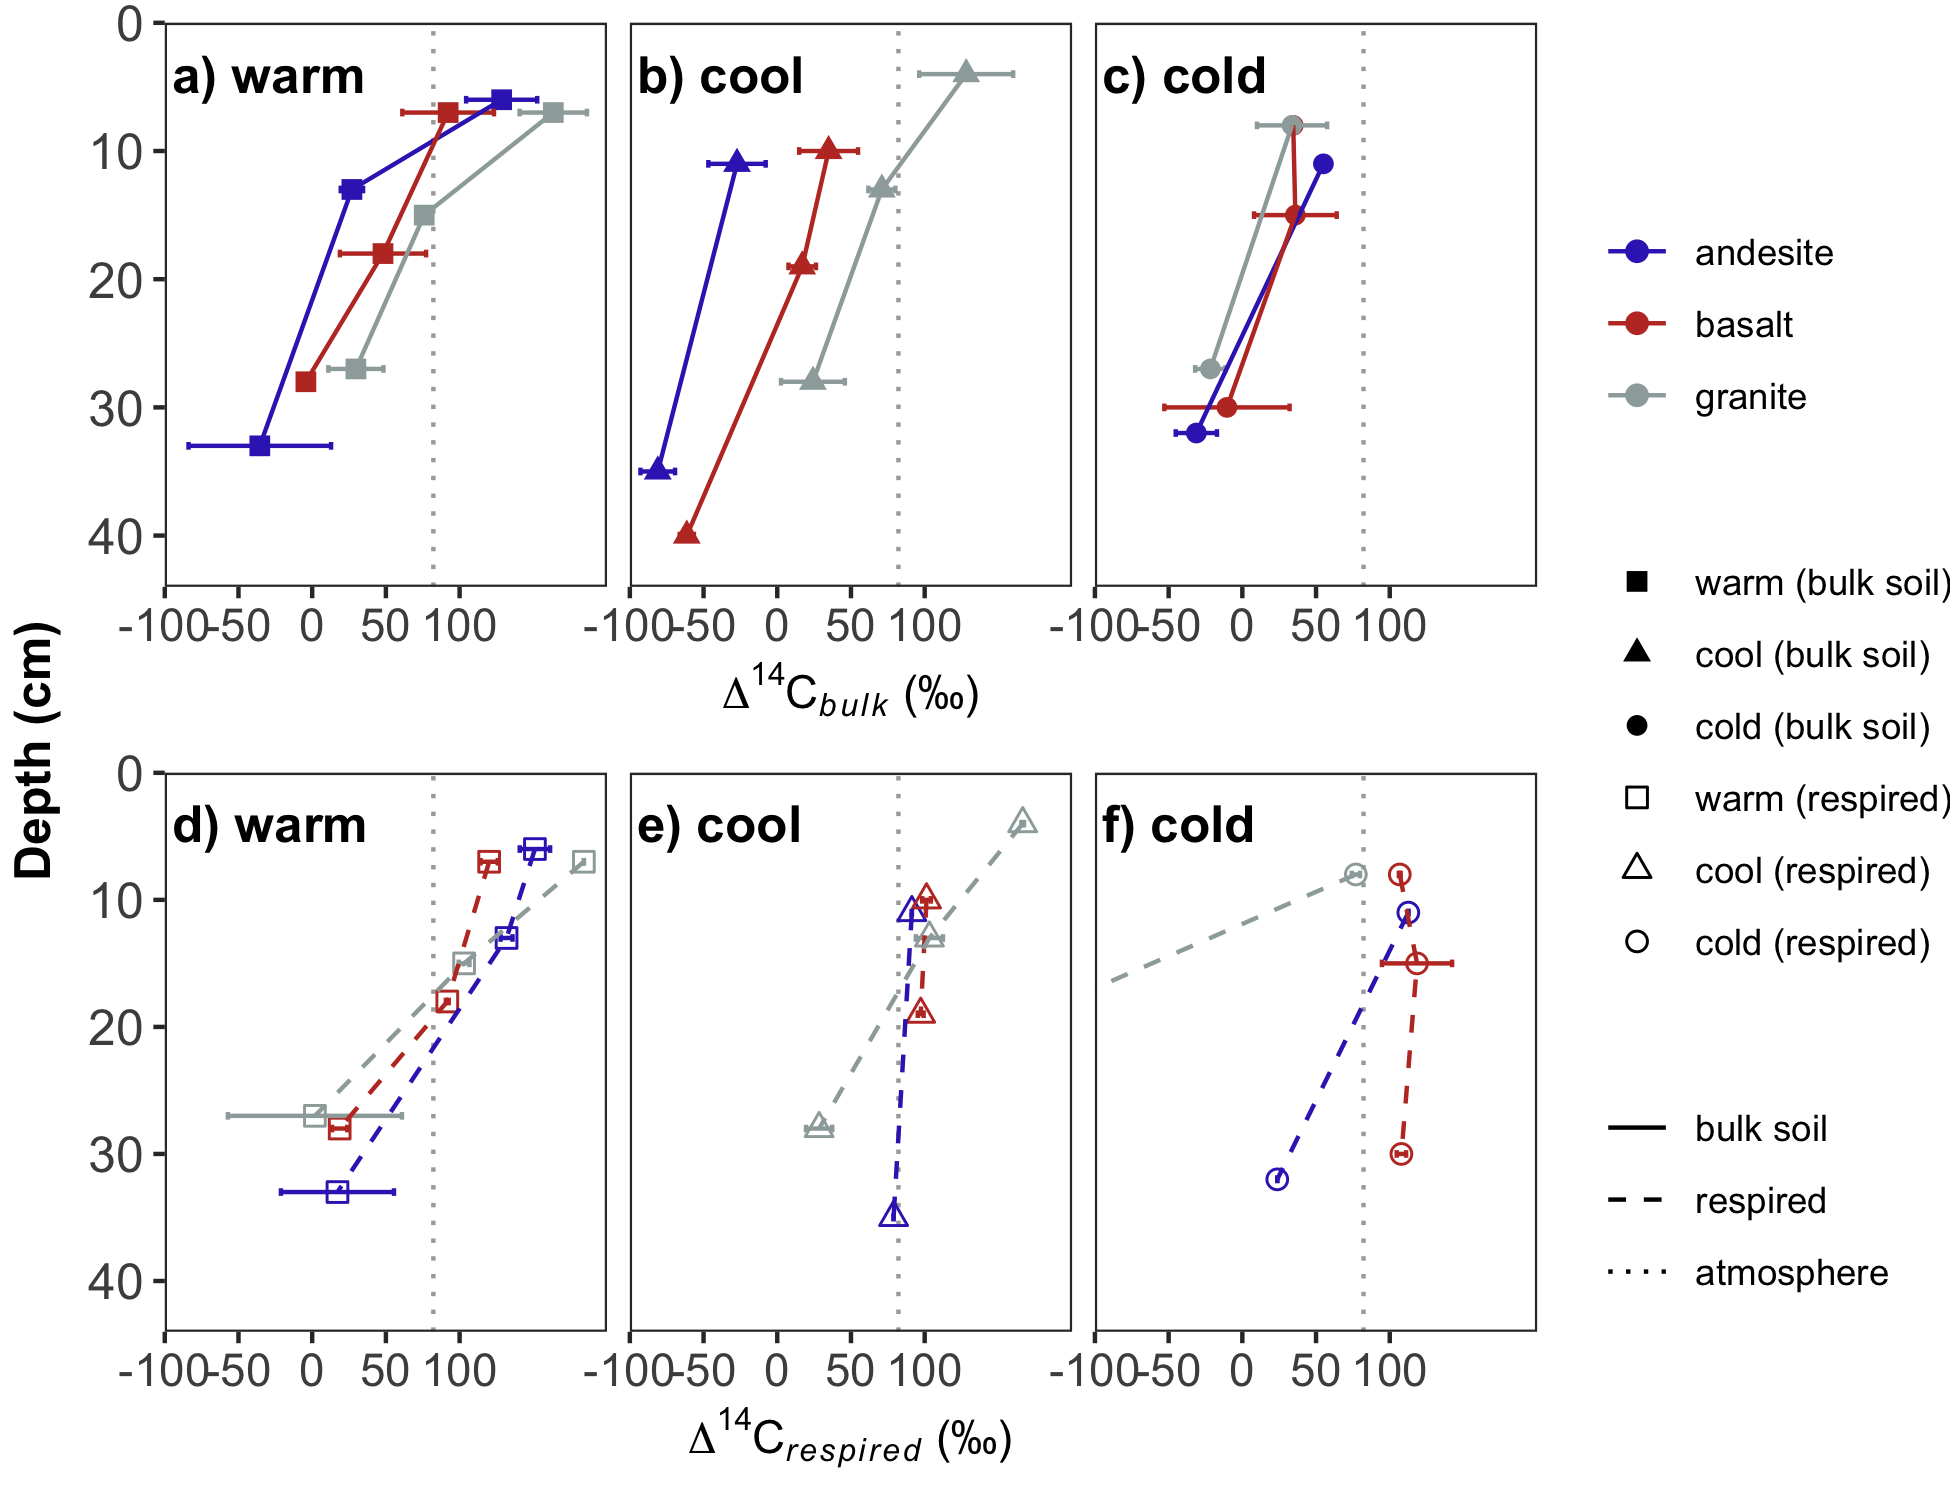
\includegraphics{sra-blk-inc-SI_files/figure-latex/plot-d14c-pro-01-1} 

}

\caption{Depth profiles of \(\Delta\)\textsuperscript{14}C\textsubscript{bulk} and \(\Delta\)\textsuperscript{14}C\textsubscript{respired} for 2001 data. Top panels show bulk data, bottom panels respired data. Panels (a) and (d) show data from the warm climate sites, (b) and (e) from the cool climate sites, and (c) and (f) from the cold climate sites. Dotted vertical lines show \(\Delta\)\textsuperscript{14}C of the atmosphere in the year of sampling. Points show the mean of three replicate profiles for bulk soil, and the mean of laboratory duplicates for respired CO\textsubscript{2}. Error bars show ±1 SD for bulk soils and the minimum and maximum for respired CO\textsubscript{2}. Respired CO\textsubscript{2} from the cold granite site (panel c) was extremely depleted in \(\Delta\)\textsuperscript{14}C and thus is excluded for display purposes.}\label{fig:plot-d14c-pro-01}
\end{figure}

\hypertarget{temporal-trend-analysis}{%
\section{Temporal trend analysis}\label{temporal-trend-analysis}}

\hypertarget{trends}{%
\subsection{Trends}\label{trends}}

Please see the main text for discussion of the temporal trends in both \(\Delta\)\textsuperscript{14}C\textsubscript{\emph{bulk}} and \(\Delta\)\textsuperscript{14}C\textsubscript{\emph{bulk}}. See SI tables \textbf{\ref{tab:blk-trend-stats}} and \textbf{\ref{tab:inc-trend-stats}} for statistics.



\begingroup\fontsize{10}{12}\selectfont

\begin{longtable}[t]{lllrlrlr}
\caption{\label{tab:blk-trend-stats}Change in \(\Delta\)\textsuperscript{14}C\textsubscript{\emph{bulk}}, 2001-2019. Degrees of freedom = 44; confidence level used = 0.95.}\\
\toprule
\multicolumn{2}{c}{ } & \multicolumn{2}{c}{0-10cm} & \multicolumn{2}{c}{10-20cm} & \multicolumn{2}{c}{20-30cm} \\
\cmidrule(l{3pt}r{3pt}){3-4} \cmidrule(l{3pt}r{3pt}){5-6} \cmidrule(l{3pt}r{3pt}){7-8}
Climate & Parent material & Trend & $SE$ & Trend & $SE$ & Trend & $SE$\\
\midrule
\endfirsthead
\caption[]{\label{tab:blk-trend-stats}Change in \(\Delta\)\textsuperscript{14}C\textsubscript{\emph{bulk}}, 2001-2019. Degrees of freedom = 44; confidence level used = 0.95. \textit{(continued)}}\\
\toprule
\multicolumn{2}{c}{ } & \multicolumn{2}{c}{0-10cm} & \multicolumn{2}{c}{10-20cm} & \multicolumn{2}{c}{20-30cm} \\
\cmidrule(l{3pt}r{3pt}){3-4} \cmidrule(l{3pt}r{3pt}){5-6} \cmidrule(l{3pt}r{3pt}){7-8}
Climate & Parent material & Trend & $SE$ & Trend & $SE$ & Trend & $SE$\\
\midrule
\endhead

\endfoot
\bottomrule
\endlastfoot
 & andesite & \textbf{-6.1} & 1.1 & -2.1 & 1.3 & 1.1 & 1.2\\
\nopagebreak
 & basalt & -1.9 & 1.1 & -0.3 & 1.3 & -1 & 1.2\\
\nopagebreak
\multirow[t]{-3}{*}{\raggedright\arraybackslash warm} & granite & \textbf{-2.8} & 1.1 & 2.1 & 1.3 & 0.2 & 1.2\\
\cmidrule{1-8}\pagebreak[0]
 & andesite & 0.1 & 1.1 & 0.4 & 1.3 & 0.3 & 1.2\\
\nopagebreak
 & basalt & -2.1 & 1.1 & \textbf{-3.7} & 1.3 & \textbf{-6.4} & 1.2\\
\nopagebreak
\multirow[t]{-3}{*}{\raggedright\arraybackslash cool} & granite & \textbf{-5} & 1.1 & \textbf{-3.7} & 1.3 & \textbf{-3.6} & 1.2\\
\cmidrule{1-8}\pagebreak[0]
 & andesite & -2.4 & 1.2 & -1.2 & 1.4 & 0.3 & 1.4\\
\nopagebreak
 & basalt & 0.8 & 1.1 & -0.4 & 1.3 & 1.6 & 1.2\\
\nopagebreak
\multirow[t]{-3}{*}{\raggedright\arraybackslash cold} & granite & -0.3 & 1.1 & 0.4 & 1.3 & 0.3 & 1.2\\*
\end{longtable}
\endgroup{}



\begingroup\fontsize{10}{12}\selectfont

\begin{longtable}[t]{lllrlrlr}
\caption{\label{tab:inc-trend-stats}Change in \(\Delta\)\textsuperscript{14}C\textsubscript{\emph{respired}}, 2001-2019. Degrees of freedom = 44; confidence level used = 0.95.}\\
\toprule
\multicolumn{2}{c}{ } & \multicolumn{2}{c}{0-10cm} & \multicolumn{2}{c}{10-20cm} & \multicolumn{2}{c}{20-30cm} \\
\cmidrule(l{3pt}r{3pt}){3-4} \cmidrule(l{3pt}r{3pt}){5-6} \cmidrule(l{3pt}r{3pt}){7-8}
Climate & Parent material & Trend & $SE$ & Trend & $SE$ & Trend & $SE$\\
\midrule
\endfirsthead
\caption[]{\label{tab:inc-trend-stats}Change in \(\Delta\)\textsuperscript{14}C\textsubscript{\emph{respired}}, 2001-2019. Degrees of freedom = 44; confidence level used = 0.95. \textit{(continued)}}\\
\toprule
\multicolumn{2}{c}{ } & \multicolumn{2}{c}{0-10cm} & \multicolumn{2}{c}{10-20cm} & \multicolumn{2}{c}{20-30cm} \\
\cmidrule(l{3pt}r{3pt}){3-4} \cmidrule(l{3pt}r{3pt}){5-6} \cmidrule(l{3pt}r{3pt}){7-8}
Climate & Parent material & Trend & $SE$ & Trend & $SE$ & Trend & $SE$\\
\midrule
\endhead

\endfoot
\bottomrule
\endlastfoot
 & andesite & \textbf{-6.2} & 0.8 & \textbf{-2.3} & 0.9 & 1.5 & 1.7\\
\nopagebreak
 & basalt & \textbf{-2.3} & 0.8 & -1.1 & 0.9 & 0.5 & 1.7\\
\nopagebreak
\multirow[t]{-3}{*}{\raggedright\arraybackslash warm} & granite & \textbf{-5} & 0.8 & 1.4 & 0.9 & 2.8 & 1.7\\
\cmidrule{1-8}\pagebreak[0]
 & andesite & -1.4 & 0.8 & -1 & 0.9 & -1.5 & 1.7\\
\nopagebreak
 & basalt & \textbf{-3.7} & 0.8 & \textbf{-6} & 0.9 & \textbf{-7.8} & 1.7\\
\nopagebreak
\multirow[t]{-3}{*}{\raggedright\arraybackslash cool} & granite & \textbf{-3.1} & 0.8 & \textbf{-4.3} & 0.9 & 0 & 1.7\\
\cmidrule{1-8}\pagebreak[0]
 & andesite & \textbf{-3} & 0.8 & -1.1 & 0.9 & 1.1 & 1.7\\
\nopagebreak
 & basalt & \textbf{-3.8} & 0.8 & \textbf{-4} & 0.9 & -3.4 & 2.1\\
\nopagebreak
\multirow[t]{-3}{*}{\raggedright\arraybackslash cold} & granite & -0.7 & 0.8 & \textbf{3.9} & 1.3 & \textbf{9.3} & 2.1\\*
\end{longtable}
\endgroup{}

\hypertarget{contrasts}{%
\subsection{Contrasts}\label{contrasts}}

We saw more significant contrasts for \(\Delta\)\textsuperscript{14}C\textsubscript{\emph{respired}} than we did for \(\Delta\)\textsuperscript{14}C\textsubscript{\emph{bulk}} (\textbf{SI Fig. \ref{tab:blk-inc-contrasts}}). When considered within climate zones, the basaltic and granitic soils were more similar to one another overall than were either to the andesitic soils. We observed parent material contrasts more commonly in the cool and cold climate sites than in the warm sites; however we only observed significant contrasts for the cold climate sites in the \(\Delta\)\textsuperscript{14}C\textsubscript{\emph{respired}} data, and not for \(\Delta\)\textsuperscript{14}C\textsubscript{\emph{bulk}}. When considered within parent materials, we saw more siginificant contrasts for the granitic and basaltic soils than for the andesitic soils (\textbf{SI Fig. \ref{tab:blk-inc-contrasts}}).



\begingroup\fontsize{10}{12}\selectfont

\begin{longtable}[t]{lllrrlrrl}
\caption{\label{tab:blk-inc-contrasts}Contrasts for bulk and respired \(\Delta\)\textsuperscript{14}C temporal trends. P value adjustment: Tukey method for comparing a family of 3 estimates.}\\
\toprule
\multicolumn{3}{c}{ } & \multicolumn{3}{c}{Bulk} & \multicolumn{3}{c}{Respired} \\
\cmidrule(l{3pt}r{3pt}){4-6} \cmidrule(l{3pt}r{3pt}){7-9}
Depth & Group & Contrast & Est. & $SE$ & $p$ & Est. & $SE$ & $p$\\
\midrule
\endfirsthead
\caption[]{\label{tab:blk-inc-contrasts}Contrasts for bulk and respired \(\Delta\)\textsuperscript{14}C temporal trends. P value adjustment: Tukey method for comparing a family of 3 estimates. \textit{(continued)}}\\
\toprule
\multicolumn{3}{c}{ } & \multicolumn{3}{c}{Bulk} & \multicolumn{3}{c}{Respired} \\
\cmidrule(l{3pt}r{3pt}){4-6} \cmidrule(l{3pt}r{3pt}){7-9}
Depth & Group & Contrast & Est. & $SE$ & $p$ & Est. & $SE$ & $p$\\
\midrule
\endhead

\endfoot
\bottomrule
\endlastfoot
 & warm & andesite - basalt & -4.2 & 1.5 & \textbf{0.023} & -3.9 & 1.2 & \textbf{0.009}\\
\nopagebreak
 & warm & andesite - granite & -3.3 & 1.5 & 0.091 &  &  & \\
\nopagebreak
 & warm & basalt - granite &  &  &  & 2.7 & 1.2 & 0.08\\
\nopagebreak
 & cool & andesite - granite & 5.0 & 1.5 & \textbf{0.005} &  &  & \\
\nopagebreak
 & cold & basalt - granite &  &  &  & -3.1 & 1.2 & \textbf{0.037}\\
\nopagebreak
 & andesite & warm - cool & -6.2 & 1.5 & \textbf{< .001} & -4.8 & 1.2 & \textbf{0.001}\\
\nopagebreak
 & andesite & warm - cold & -3.7 & 1.6 & 0.064 & -3.3 & 1.2 & \textbf{0.029}\\
\nopagebreak
 & granite & warm - cold &  &  &  & -4.2 & 1.2 & \textbf{0.005}\\
\nopagebreak
\multirow[t]{-9}{*}{\raggedright\arraybackslash 0-10cm} & granite & cool - cold & -4.7 & 1.5 & \textbf{0.01} &  &  & \\
\cmidrule{1-9}\pagebreak[0]
 & warm & andesite - granite & -4.2 & 1.8 & 0.055 & -3.7 & 1.3 & \textbf{0.029}\\
\nopagebreak
 & cool & andesite - basalt & 4.1 & 1.8 & 0.065 & 4.9 & 1.3 & \textbf{0.004}\\
\nopagebreak
 & cool & andesite - granite & 4.1 & 1.8 & 0.068 & 3.3 & 1.3 & 0.055\\
\nopagebreak
 & cold & andesite - basalt &  &  &  & 2.9 & 1.3 & 0.097\\
\nopagebreak
 & cold & andesite - granite &  &  &  & -5.0 & 1.6 & \textbf{0.015}\\
\nopagebreak
 & cold & basalt - granite &  &  &  & -7.9 & 1.6 & \textbf{< .001}\\
\nopagebreak
 & basalt & warm - cool &  &  &  & 4.8 & 1.3 & \textbf{0.005}\\
\nopagebreak
 & basalt & warm - cold &  &  &  & 2.9 & 1.3 & 0.097\\
\nopagebreak
 & granite & warm - cool & 5.8 & 1.8 & \textbf{0.006} & 5.7 & 1.3 & \textbf{0.001}\\
\nopagebreak
\multirow[t]{-10}{*}{\raggedright\arraybackslash 10-20cm} & granite & cool - cold & -4.1 & 1.8 & 0.066 & -8.1 & 1.6 & \textbf{< .001}\\
\cmidrule{1-9}\pagebreak[0]
 & cool & andesite - basalt & 6.7 & 1.7 & \textbf{0.001} & 6.3 & 2.5 & 0.054\\
\nopagebreak
 & cool & andesite - granite & 3.9 & 1.7 & 0.072 &  &  & \\
\nopagebreak
 & cool & basalt - granite &  &  &  & -7.8 & 2.5 & \textbf{0.016}\\
\nopagebreak
 & cold & andesite - granite &  &  &  & -8.1 & 2.8 & \textbf{0.025}\\
\nopagebreak
 & cold & basalt - granite &  &  &  & -12.7 & 3.0 & \textbf{0.002}\\
\nopagebreak
 & basalt & warm - cool & 5.5 & 1.7 & \textbf{0.009} & 8.3 & 2.5 & \textbf{0.011}\\
\nopagebreak
 & basalt & cool - cold & -8.0 & 1.7 & \textbf{< .001} &  &  & \\
\nopagebreak
 & granite & warm - cool & 3.8 & 1.7 & 0.085 &  &  & \\
\nopagebreak
 & granite & warm - cold &  &  &  & -6.5 & 2.8 & 0.077\\
\nopagebreak
\multirow[t]{-10}{*}{\raggedright\arraybackslash 20-30cm} & granite & cool - cold & -3.9 & 1.7 & 0.072 & -9.3 & 2.8 & \textbf{0.011}\\*
\end{longtable}
\endgroup{}

\hypertarget{mineral-assemblages}{%
\section{Mineral assemblages}\label{mineral-assemblages}}

\textbf{SI Figs. \ref{fig:min-all-blk-inc-plot}}, \textbf{\ref{fig:min-blk30-plot}}, and \textbf{\ref{fig:min-inc30-plot}}.



\begin{figure}

{\centering 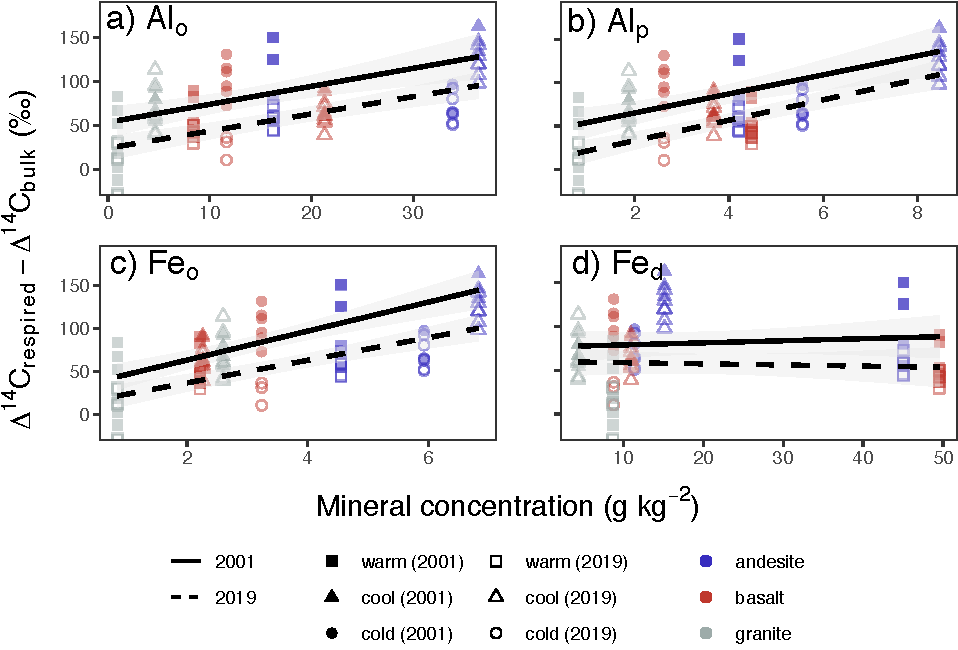
\includegraphics{sra-blk-inc-SI_files/figure-latex/min-all-blk-inc-plot-1} 

}

\caption{Relationship of selectively dissolved iron and alumnimum to the difference between \(\Delta\)\textsuperscript{14}C\textsubscript{\emph{respired}} and \(\Delta\)\textsuperscript{14}C\textsubscript{\emph{bulk}} (\(\Delta\)\textsuperscript{14}C\textsubscript{\emph{respired-bulk}}). \textsuperscript{a)} Oxalate-extractable aluminum, \textsuperscript{b)} Pyrophosphate-extractable aluminum, \textsuperscript{c)} Oxalate-extractable iron) \textsuperscript{d)} Dithionite-extractable iron. Points show mass-weighted mineral concentrations and carbon-weighted values of \(\Delta\)\textsuperscript{14}C\textsubscript{\emph{respired-bulk}} for 0-30cm profiles. Lines show linear model fits from \textbf{Eq. 5}.}\label{fig:min-all-blk-inc-plot}
\end{figure}



\begin{figure}

{\centering 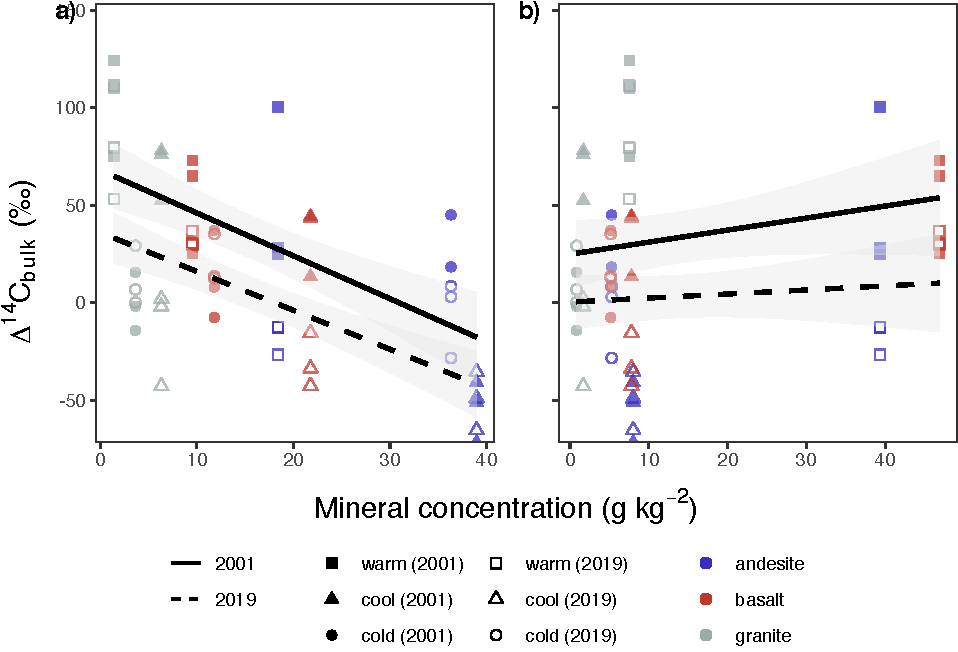
\includegraphics{sra-blk-inc-SI_files/figure-latex/min-blk30-plot-1} 

}

\caption{Relationship of poorly crystalline and crystalline minerals to \(\Delta\)\textsuperscript{14}C\textsubscript{\emph{bulk}}. \textsuperscript{a)} Poorly crystalline mineral content (oxalate-extractable aluminum + 1/2 oxalate-extractable iron), \textsuperscript{b)} Crystalline mineral content (dithionite-extractable iron - oxalate-extractable iron). Points show mass-weighted mineral concentrations and carbon-weighted values of \(\Delta\)\textsuperscript{14}C\textsubscript{\emph{bulk}} for 0-30cm profiles. Lines show linear model fits from \textbf{Eq. 5}.}\label{fig:min-blk30-plot}
\end{figure}



\begin{figure}

{\centering 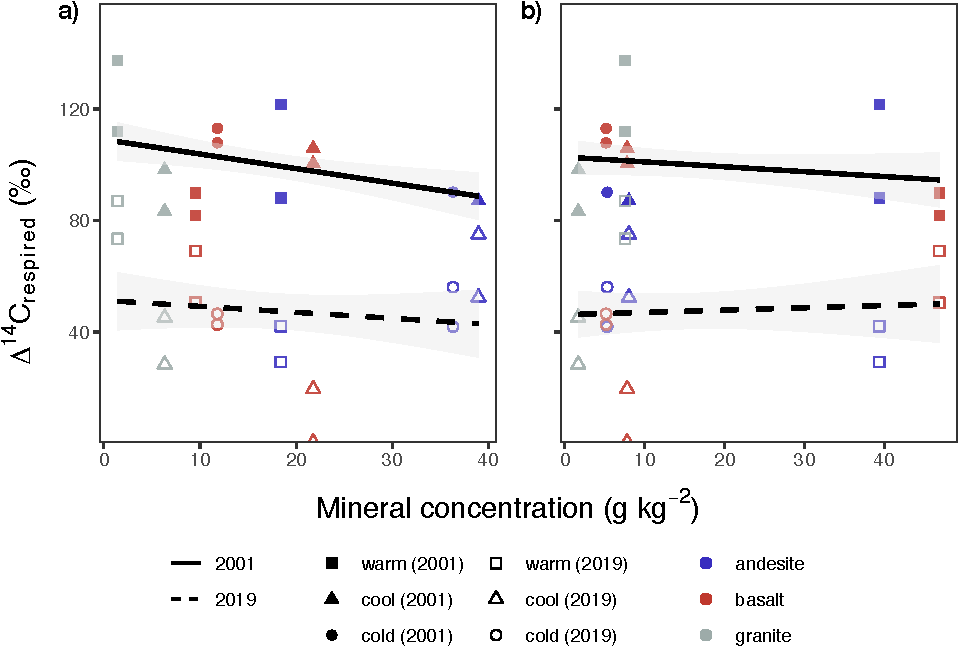
\includegraphics{sra-blk-inc-SI_files/figure-latex/min-inc30-plot-1} 

}

\caption{Relationship of poorly crystalline and crystalline minerals to \(\Delta\)\textsuperscript{14}C\textsubscript{\emph{respired}}. \textsuperscript{a)} Poorly crystalline mineral content (oxalate-extractable aluminum + 1/2 oxalate-extractable iron), \textsuperscript{b)} Crystalline mineral content (dithionite-extractable iron - oxalate-extractable iron). Points show mass-weighted mineral concentrations and carbon-weighted values of \(\Delta\)\textsuperscript{14}C\textsubscript{\emph{respired}} for 0-30cm profiles. Lines show linear model fits from \textbf{Eq. 5}.}\label{fig:min-inc30-plot}
\end{figure}


\clearpage
\renewcommand{\listfigurename}{Figure captions}

\clearpage
\renewcommand{\listtablename}{Table captions}


\end{document}
